% Options for packages loaded elsewhere
\PassOptionsToPackage{unicode}{hyperref}
\PassOptionsToPackage{hyphens}{url}
\PassOptionsToPackage{dvipsnames,svgnames,x11names}{xcolor}
%
\documentclass[
  letterpaper,
  DIV=11,
  numbers=noendperiod]{scrreprt}

\usepackage{amsmath,amssymb}
\usepackage{lmodern}
\usepackage{iftex}
\ifPDFTeX
  \usepackage[T1]{fontenc}
  \usepackage[utf8]{inputenc}
  \usepackage{textcomp} % provide euro and other symbols
\else % if luatex or xetex
  \usepackage{unicode-math}
  \defaultfontfeatures{Scale=MatchLowercase}
  \defaultfontfeatures[\rmfamily]{Ligatures=TeX,Scale=1}
\fi
% Use upquote if available, for straight quotes in verbatim environments
\IfFileExists{upquote.sty}{\usepackage{upquote}}{}
\IfFileExists{microtype.sty}{% use microtype if available
  \usepackage[]{microtype}
  \UseMicrotypeSet[protrusion]{basicmath} % disable protrusion for tt fonts
}{}
\makeatletter
\@ifundefined{KOMAClassName}{% if non-KOMA class
  \IfFileExists{parskip.sty}{%
    \usepackage{parskip}
  }{% else
    \setlength{\parindent}{0pt}
    \setlength{\parskip}{6pt plus 2pt minus 1pt}}
}{% if KOMA class
  \KOMAoptions{parskip=half}}
\makeatother
\usepackage{xcolor}
\setlength{\emergencystretch}{3em} % prevent overfull lines
\setcounter{secnumdepth}{5}
% Make \paragraph and \subparagraph free-standing
\ifx\paragraph\undefined\else
  \let\oldparagraph\paragraph
  \renewcommand{\paragraph}[1]{\oldparagraph{#1}\mbox{}}
\fi
\ifx\subparagraph\undefined\else
  \let\oldsubparagraph\subparagraph
  \renewcommand{\subparagraph}[1]{\oldsubparagraph{#1}\mbox{}}
\fi


\providecommand{\tightlist}{%
  \setlength{\itemsep}{0pt}\setlength{\parskip}{0pt}}\usepackage{longtable,booktabs,array}
\usepackage{calc} % for calculating minipage widths
% Correct order of tables after \paragraph or \subparagraph
\usepackage{etoolbox}
\makeatletter
\patchcmd\longtable{\par}{\if@noskipsec\mbox{}\fi\par}{}{}
\makeatother
% Allow footnotes in longtable head/foot
\IfFileExists{footnotehyper.sty}{\usepackage{footnotehyper}}{\usepackage{footnote}}
\makesavenoteenv{longtable}
\usepackage{graphicx}
\makeatletter
\def\maxwidth{\ifdim\Gin@nat@width>\linewidth\linewidth\else\Gin@nat@width\fi}
\def\maxheight{\ifdim\Gin@nat@height>\textheight\textheight\else\Gin@nat@height\fi}
\makeatother
% Scale images if necessary, so that they will not overflow the page
% margins by default, and it is still possible to overwrite the defaults
% using explicit options in \includegraphics[width, height, ...]{}
\setkeys{Gin}{width=\maxwidth,height=\maxheight,keepaspectratio}
% Set default figure placement to htbp
\makeatletter
\def\fps@figure{htbp}
\makeatother
\newlength{\cslhangindent}
\setlength{\cslhangindent}{1.5em}
\newlength{\csllabelwidth}
\setlength{\csllabelwidth}{3em}
\newlength{\cslentryspacingunit} % times entry-spacing
\setlength{\cslentryspacingunit}{\parskip}
\newenvironment{CSLReferences}[2] % #1 hanging-ident, #2 entry spacing
 {% don't indent paragraphs
  \setlength{\parindent}{0pt}
  % turn on hanging indent if param 1 is 1
  \ifodd #1
  \let\oldpar\par
  \def\par{\hangindent=\cslhangindent\oldpar}
  \fi
  % set entry spacing
  \setlength{\parskip}{#2\cslentryspacingunit}
 }%
 {}
\usepackage{calc}
\newcommand{\CSLBlock}[1]{#1\hfill\break}
\newcommand{\CSLLeftMargin}[1]{\parbox[t]{\csllabelwidth}{#1}}
\newcommand{\CSLRightInline}[1]{\parbox[t]{\linewidth - \csllabelwidth}{#1}\break}
\newcommand{\CSLIndent}[1]{\hspace{\cslhangindent}#1}

\KOMAoption{captions}{tableheading}
\makeatletter
\makeatother
\makeatletter
\@ifpackageloaded{bookmark}{}{\usepackage{bookmark}}
\makeatother
\makeatletter
\@ifpackageloaded{caption}{}{\usepackage{caption}}
\AtBeginDocument{%
\ifdefined\contentsname
  \renewcommand*\contentsname{Table of contents}
\else
  \newcommand\contentsname{Table of contents}
\fi
\ifdefined\listfigurename
  \renewcommand*\listfigurename{List of Figures}
\else
  \newcommand\listfigurename{List of Figures}
\fi
\ifdefined\listtablename
  \renewcommand*\listtablename{List of Tables}
\else
  \newcommand\listtablename{List of Tables}
\fi
\ifdefined\figurename
  \renewcommand*\figurename{Figure}
\else
  \newcommand\figurename{Figure}
\fi
\ifdefined\tablename
  \renewcommand*\tablename{Table}
\else
  \newcommand\tablename{Table}
\fi
}
\@ifpackageloaded{float}{}{\usepackage{float}}
\floatstyle{ruled}
\@ifundefined{c@chapter}{\newfloat{codelisting}{h}{lop}}{\newfloat{codelisting}{h}{lop}[chapter]}
\floatname{codelisting}{Listing}
\newcommand*\listoflistings{\listof{codelisting}{List of Listings}}
\makeatother
\makeatletter
\@ifpackageloaded{caption}{}{\usepackage{caption}}
\@ifpackageloaded{subcaption}{}{\usepackage{subcaption}}
\makeatother
\makeatletter
\@ifpackageloaded{tcolorbox}{}{\usepackage[many]{tcolorbox}}
\makeatother
\makeatletter
\@ifundefined{shadecolor}{\definecolor{shadecolor}{rgb}{.97, .97, .97}}
\makeatother
\makeatletter
\makeatother
\ifLuaTeX
  \usepackage{selnolig}  % disable illegal ligatures
\fi
\IfFileExists{bookmark.sty}{\usepackage{bookmark}}{\usepackage{hyperref}}
\IfFileExists{xurl.sty}{\usepackage{xurl}}{} % add URL line breaks if available
\urlstyle{same} % disable monospaced font for URLs
\hypersetup{
  pdftitle={Cours management de la donnée},
  pdfauthor={Anne-Laure Donzel},
  colorlinks=true,
  linkcolor={blue},
  filecolor={Maroon},
  citecolor={Blue},
  urlcolor={Blue},
  pdfcreator={LaTeX via pandoc}}

\title{Cours management de la donnée}
\author{Anne-Laure Donzel}
\date{17/10/2023}

\begin{document}
\maketitle
\ifdefined\Shaded\renewenvironment{Shaded}{\begin{tcolorbox}[boxrule=0pt, interior hidden, borderline west={3pt}{0pt}{shadecolor}, sharp corners, frame hidden, breakable, enhanced]}{\end{tcolorbox}}\fi

\renewcommand*\contentsname{Table of contents}
{
\hypersetup{linkcolor=}
\setcounter{tocdepth}{2}
\tableofcontents
}
\bookmarksetup{startatroot}

\hypertarget{pruxe9face}{%
\chapter*{Préface}\label{pruxe9face}}
\addcontentsline{toc}{chapter}{Préface}

Ce cours s'inscrit dans le Master Politiques Sociales de l'Université
d'Avignon. Il cherche à apporter des réponses aux besoins de
professionnalisation et de qualification des cadres du social et du
sanitaire \& social.

Il s'intitule ``Data management et data visualisation''. Mais en quoi
ces sujets peuvent contribuer à la formation des futur·es cadres et
professionnel·les du secteur sanitaire \& social ?

Le sujet de la donnée est aujourd'hui omniprésent dans les organisations
: elles sont collectées, analysées, observées et elles viennent
éclairer, influer, orienter les décisions, tans dans le secteur public
que dans le secteur privé.

Comment organiser cette bonne gestion des données et que peut-on en
faire sont aujourd'hui des questions importantes et il est nécessaire
d'avoir quelques clés de compréhension et d'analyse de données.

Ce cours ne sera pas centré sur la protection des données personnelles,
ni sur les données de santé. Il ne sera pas non plus un cours technique
sur le code.

\bookmarksetup{startatroot}

\hypertarget{programme}{%
\chapter{Programme}\label{programme}}

\begin{enumerate}
\def\labelenumi{\arabic{enumi}.}
\item
  Séance 1 : La politique de la donnée en France **fresque**

  \begin{enumerate}
  \def\labelenumii{\arabic{enumii}.}
  \item
    Retour sur la notion de donnée
  \item
    Rappels règlementaires
  \item
    Les tendances de la politique de la donnée : open data, open gov,
    règlementation européenne\ldots{}
  \end{enumerate}
\item
  Séance 2 : Rendre visible l'invisible : apport de la dataviz

  \begin{enumerate}
  \def\labelenumii{\arabic{enumii}.}
  \item
    Historique de la représentation visuelle

    \begin{itemize}
    \item
      Selon vous : de quand date la première représentation visuelle ?
    \item
      Les différents types de représentation
    \item
      Quelques grands noms : Nightingale, DuBois
    \end{itemize}
  \item
    Le meilleur et le pire (exercice critique)
  \end{enumerate}
\item
  Séance 3 : Des données au services des politiques publiques
\end{enumerate}

\begin{verbatim}
1.  Panorama du management des données dans le secteur public (en particulier les CD)

2.  Enjeux du data management

3.  Cycle de vie des données

4.  Organisation interne
\end{verbatim}

\begin{enumerate}
\def\labelenumi{\arabic{enumi}.}
\setcounter{enumi}{3}
\item
  Séance 4 : Observer, piloter, contrôler

  \begin{enumerate}
  \def\labelenumii{\arabic{enumii}.}
  \tightlist
  \item
    Exercice critique des politiques publiques pilotées par la donnée
  \end{enumerate}
\item
  Séance 5 : Restitution des travaux de groupe
\end{enumerate}

\bookmarksetup{startatroot}

\hypertarget{syllabus}{%
\chapter{Syllabus}\label{syllabus}}

\bookmarksetup{startatroot}

\hypertarget{evaluation}{%
\chapter{Evaluation}\label{evaluation}}

\hypertarget{modalituxe9s-de-contruxf4le-de-connaissance}{%
\section{Modalités de contrôle de
connaissance}\label{modalituxe9s-de-contruxf4le-de-connaissance}}

Un rendu écrit sous la forme d'une infographie ou affiche (50\%) qui
fera l'objet d'une présentation orale (25\%) et une note sur la
participation et l'assiduité (25\%).

\hypertarget{sur-quoi-serez-vous-notuxe9}{%
\subsection{Sur quoi serez vous noté
?}\label{sur-quoi-serez-vous-notuxe9}}

En groupe de 3 ou 4, vous allez devoir présenter une
\textbf{controverse} en l'illustrant avec des données que vous pourrez
trouver lors de vos recherches. Le tout sur un sujet concernant les
politiques sociales.

\textbf{\emph{A l'oral :}}

\begin{itemize}
\item
  Sur la bonne répartition de votre temps de parole (tous les membres du
  groupe devront intervenir).
\item
  Sur la clarté et la cohérence de votre déroulé.
\item
  Sur la formulation de votre controverse.
\item
  Sur la façon dont vous éviterez de lire votre affiche : à l'oral,
  l'affiche sera un support mais vous devrez aller plus loin en
  proposant une présentation plus exhaustive et plus complète.
\item
  Chaque groupe sera aussi noté sur les questions et réactions aux
  travaux des autres groupes.
\item
  Sur votre capacité à faire le lien entre votre controverse et les
  éléments du cours.
\item
  Sur la variété de vos sources.
\end{itemize}

\textbf{\emph{A l'écrit :}}

\begin{itemize}
\item
  Sur votre synthèse du sujet.
\item
  Sur la formulation de votre controverse.
\item
  La forme comptera également mais ce ne sera pas l'élément essentiel
  (vous n'êtes pas graphiste).
\end{itemize}

\hypertarget{cest-quoi-une-controverse}{%
\section{C'est quoi une controverse ?}\label{cest-quoi-une-controverse}}

Vous trouverez des exemples
\href{https://www.controverses-esiee.fr/archive/}{là}. En quelques mots,
vous allez devoir analyser un sujet en tenant compte des différents
argumentaires et points de vue qui peuvent exister. Pour qu'il y ait
controverse, il faut du débat, des données et des arguments.

Pour cela, vous devrez mobiliser et exploiter des articles de presse,
des émissions, des podcasts\ldots{}

\hypertarget{quels-sont-les-livrables-attendus}{%
\subsection{Quels sont les livrables attendus
?}\label{quels-sont-les-livrables-attendus}}

Un livrable écrit sous la forme d'une affiche ou d'une infographie de
synthèse, elle devra contenir les éléments suivants :

\begin{itemize}
\item
  Le rappel du titre de votre controverse
\item
  Le contexte : quelle est la controverse ? d'où vient elle ?
\item
  Des chiffres clés (pensez dataviz !)
\item
  Les enjeux (en quoi la controverse est-elle importante ?)
\item
  La cartographie de la controverse : c'est un point important, c'est le
  coeur de votre controverse. Sous une forme visuelle (par exemple une
  mind map), vous devez indiquer qui est pour, qui est contre (il peut
  s'agir de personnes ou d'organismes) et les liens éventuels entre ces
  acteurs.
\item
  Une ou plusieurs sections avec : la date, les noms de vos équipiers
\end{itemize}

Lors de la dernière séance, vous présenterez à l'oral cette controverse.
Vous devrez à ce moment présenter de façon plus complète votre travail.
Par exemple avec :

\begin{itemize}
\item
  Les concepts clés (terminologie, schémas)
\item
  Des citations (« verbatims »)
\item
  Une explication méthodologique : comment vous êtes vous réparti le
  travail ? quelles difficultés avez vous rencontrés ?
\item
  Des remerciements si vous avez réussi à interviewer ou correspondre
  avec des acteurs.
\end{itemize}

\hypertarget{exemples-de-thuxe9matiques}{%
\subsection{Exemples de thématiques}\label{exemples-de-thuxe9matiques}}

Ce ne sont que des exemples de sujets, vous pouvez en proposer d'autres
! Dans votre questionnement, il devra toujours y avoir une dimension
``données''.

\begin{itemize}
\item
  La lutte contre le non recours aux droits
\item
  L'IA au service de la santé
\item
  Centraliser les données de santé : le Health Data Hub
\item
  Les données et l'inclusion numérique
\item
  Les données et la crise COVID
\item
  Ouverture des données du secteur sanitaire et social
\item
  L'évaluation des politiques publiques
\item
  IA générative et politique sociale
\end{itemize}

\hypertarget{quelques-conseils}{%
\subsection{Quelques conseils}\label{quelques-conseils}}

\hypertarget{par-ouxf9-duxe9marrer}{%
\subsubsection{Par où démarrer ?}\label{par-ouxf9-duxe9marrer}}

\begin{itemize}
\item
  Choisir un sujet et le formuler comme une question de débat. Par ex.,
  sur la thématique ``La lutte contre le non recours aux droits'' peut
  être formulée de la façon suivante : ``Les données peuvent-elles aider
  dans la lutte contre le non recours aux droits ?''.
\item
  Rechercher des articles, des émissions sur le sujet, notez bien vos
  sources.
\item
  Travailler sur le contexte : rechercher des chiffres clés, les grandes
  dates etc\ldots{}
\end{itemize}

\hypertarget{ruxe9aliser-la-cartographie}{%
\subsubsection{Réaliser la
cartographie}\label{ruxe9aliser-la-cartographie}}

\begin{itemize}
\item
  Identifier les acteurs et leur positionnement : vous pouvez tenir un
  fichier avec les acteurs, ses arguments, son type (personne,
  association, ONG, entreprise\ldots).
\item
  Positionner les acteurs sur la matrice suivante pour vous aider à
  réaliser la
  cartographie\includegraphics{./images/acteurs_cartographie.jpg}
\item
  Réaliser votre support visuel
\end{itemize}

\hypertarget{quelques-outils-pour-vous-aider}{%
\subsection{Quelques outils pour vous
aider}\label{quelques-outils-pour-vous-aider}}

- \href{https://www.canva.com/}{Canva}

- \href{https://piktochart.com/}{Piktochart}

- \href{https://www.visme.co/make-infographics/}{Visme}

- \href{https://www.easel.ly/}{Easel.ly}

- Ou un bon vieux Powerpoint

\bookmarksetup{startatroot}

\hypertarget{suxe9ance-1---introduction-uxe0-la-donnuxe9e}{%
\chapter{Séance 1 - Introduction à la
donnée}\label{suxe9ance-1---introduction-uxe0-la-donnuxe9e}}

\hypertarget{objectifs-de-la-suxe9ance}{%
\section{Objectifs de la séance}\label{objectifs-de-la-suxe9ance}}

\begin{itemize}
\item
  Connaître les origines historiques des politiques de la donnée en
  France
\item
  Connaître les grands principes de l'ouverture et du partage des
  données
\item
  Connaître le cadre juridique de la politique de la donnée
\item
  Comprendre la place de l'ouverture des données dans la modernisation
  de l'administration
\item
  Comprendre les bénéfices du partage de données en s'appropriant des
  cas d'usages
\end{itemize}

\hypertarget{support-de-la-suxe9ance}{%
\section{Support de la séance}\label{support-de-la-suxe9ance}}

Lien vers la présentation de l'exercice de fresque :

\includegraphics{./images/Séance 1 - 7 février 2024.pdf}

Lien vers le livret de synthèse :

\begin{figure}

{\centering \includegraphics{./images/Fresque - livret.pdf}

}

\end{figure}

\hypertarget{productions}{%
\section{Productions}\label{productions}}

{[}A venir après la séance{]}

\bookmarksetup{startatroot}

\hypertarget{suxe9ance-2---repruxe9senter-le-monde-une-longue-histoire}{%
\chapter{Séance 2 - Représenter le monde : une longue
histoire}\label{suxe9ance-2---repruxe9senter-le-monde-une-longue-histoire}}

\hypertarget{support-cours}{%
\section{Support cours}\label{support-cours}}

\begin{figure}

{\centering 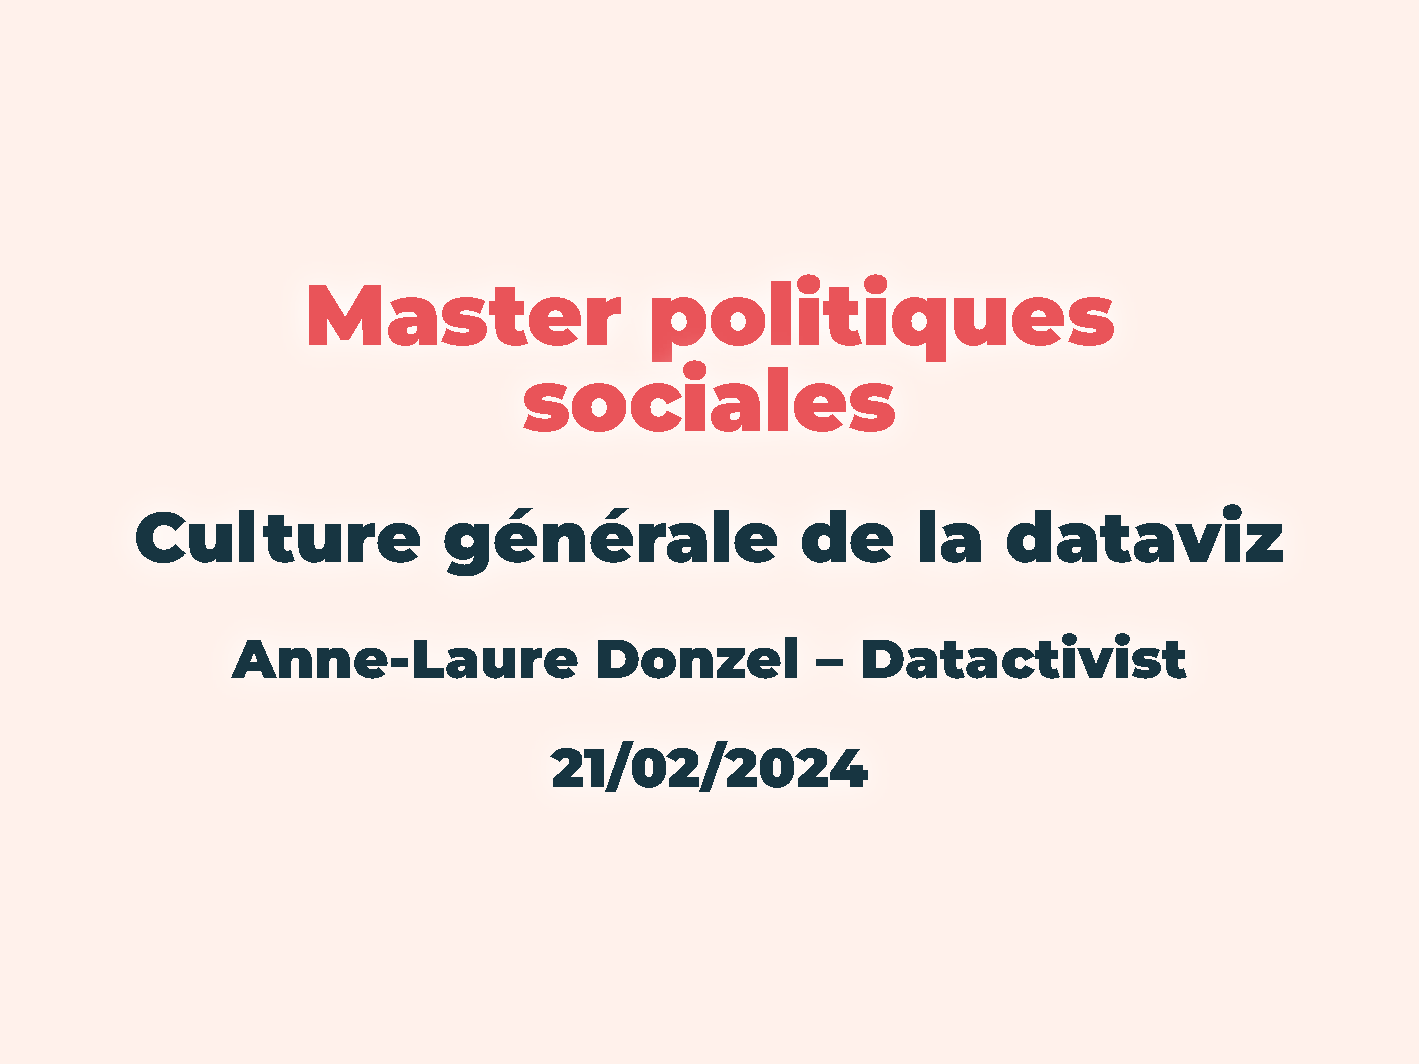
\includegraphics{./images/seance2_dataviz_coursUAPV.pdf}

}

\end{figure}

\hypertarget{activituxe9s}{%
\section{Activités}\label{activituxe9s}}

\hypertarget{activituxe9-1}{%
\subsection{Activité 1}\label{activituxe9-1}}

A votre avis de quand date la plus ancienne représentation graphique
d'un phénomène ?

\hypertarget{activituxe9-2}{%
\subsection{Activité 2}\label{activituxe9-2}}

Former 4 groupes, chaque groupe va analyser une des datavisualisations
qui se trouvent ci-dessous.

Vous allez avoir 45 minutes pour l'analyse, sur les points suivants :

\begin{itemize}
\item
  Présentez l'auteur·ice de cette datavisualisation ?
\item
  De quand date cette datavisualisation et dans quel contexte a t elle
  été créée ?
\item
  Que cherche à nous dire cette datavisualisation ?
\item
  Quel est le mode de représentation choisie ?
\item
  Quelles sont les données d'origine ?
\item
  Qu'est-ce qui vous interpelle ou étonne ?
\end{itemize}

Pour cela : complétez, en groupe, le
\href{https://digipad.app/p/619238/1ccf04fb11e13}{pad}

\begin{enumerate}
\def\labelenumi{\arabic{enumi}.}
\item
  Florence Nightingale, Public domain, via Wikimedia Commons :
  \href{https://upload.wikimedia.org/wikipedia/commons/1/17/Nightingale-mortality.jpg}{``Diagram
  of the causes of mortality in the army in the East'' (1858) by
  Florence Nightingale, a colored pie chart to illustrate causes of
  death in the British Army}

  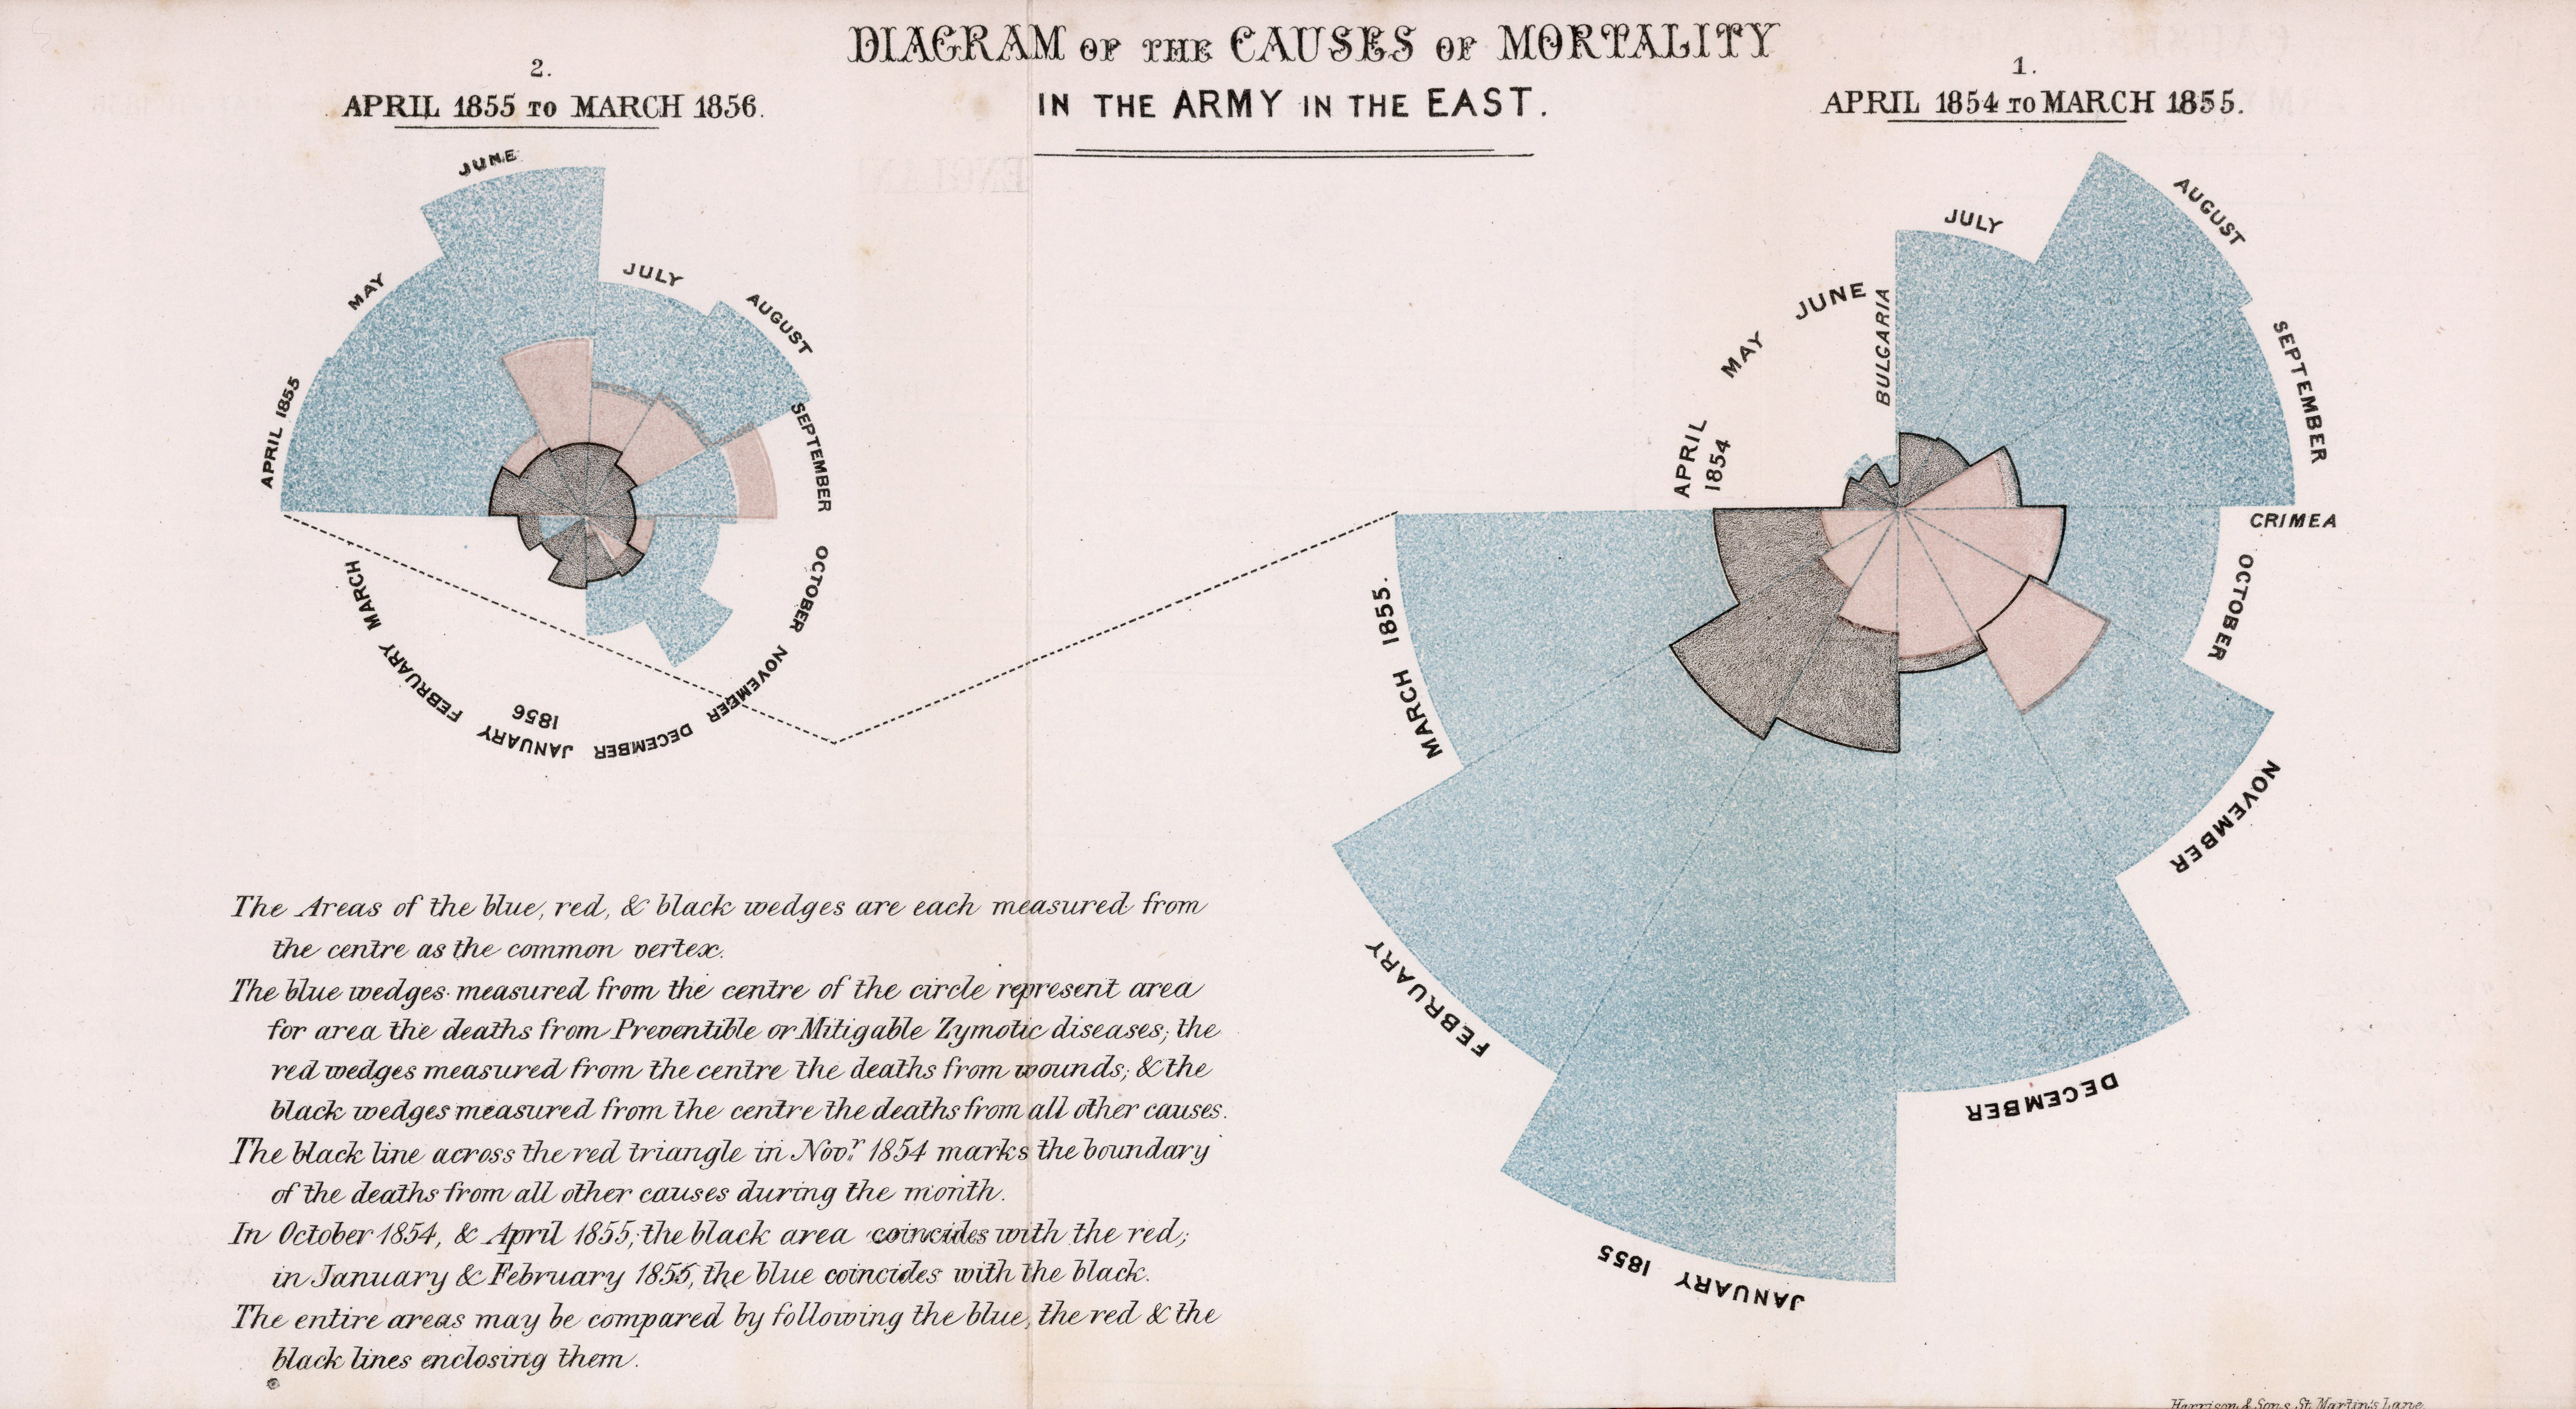
\includegraphics{./images/Nightingale-mortality.jpg}
\item
  W.E.B DuBois, African American Photographs Assembled for 1900 Paris
  Exposition, Public domain, via Wikimedia Commons :
  \href{https://commons.wikimedia.org/wiki/File:The_Georgia_Negro_LCCN2013650429.jpg}{Graph
  shows marital status by age of African Americans compared to Germans}

  \includegraphics{./images/The_Georgia_Negro_LCCN2013650429.jpg}
\item
  John Snow, Public domain, via Wikimedia Commons :
  \href{https://en.wikipedia.org/wiki/File:Snow-cholera-map-1.jpg\#/media/File:Snow-cholera-map-1.jpg}{Map
  of the book ``On the Mode of Communication of Cholera'' by John Snow,
  originally published in 1854 by C.F. Cheffins, Lith, Southhampton
  Buildings, London,
  England}\includegraphics{./images/Snow-cholera-map-1.jpg}
\item
  Charles Joseph Minard, Public domain, via Wikimedia Commons :
  \href{https://commons.wikimedia.org/wiki/File:Minard.png\#/media/Fichier:Minard.png}{Carte
  figurative des pertes successives en hommes de l'Armée française dans
  la campagne de Russie en 1812-1813}

  \includegraphics{./images/Minard.png}
\end{enumerate}

\hypertarget{activituxe9-3}{%
\subsection{Activité 3}\label{activituxe9-3}}

En groupe, analisez les visualisations présentes sur le pad, qu'en
pensez-vous ?

\hypertarget{point-sur-le-projet-final}{%
\section{Point sur le projet final}\label{point-sur-le-projet-final}}

Cette semaine vous devez :

\begin{itemize}
\item
  Avoir constitué votre groupe ✅
\item
  Avoir trouvé votre sujet ✅
\end{itemize}

\hypertarget{ressources}{%
\section{Ressources}\label{ressources}}

\href{https://www.youtube.com/watch?v=N00g9Q9stBo}{A brief history of
datavisualisation}

\href{https://www.datavis.ca/gallery/}{Des bonnes et des mauvaises
pratiques}

\bookmarksetup{startatroot}

\hypertarget{suxe9ance-3}{%
\chapter{Séance 3}\label{suxe9ance-3}}

\hypertarget{support-de-la-suxe9ance-1}{%
\section{Support de la séance}\label{support-de-la-suxe9ance-1}}

\hypertarget{activituxe9s-1}{%
\section{Activités}\label{activituxe9s-1}}

\hypertarget{ressources-1}{%
\section{Ressources}\label{ressources-1}}

https://www.resovilles.com/wp-content/uploads/2022/09/Data\_et\_quartiers-le\_livre\_blanc-web-19-09-light-1.pdf

Rapport data et territoire

\bookmarksetup{startatroot}

\hypertarget{suxe9ance-4}{%
\chapter{Séance 4}\label{suxe9ance-4}}

\bookmarksetup{startatroot}

\hypertarget{suxe9ance-5}{%
\chapter{Séance 5}\label{suxe9ance-5}}

\bookmarksetup{startatroot}

\hypertarget{suxe9ance-6}{%
\chapter{Séance 6}\label{suxe9ance-6}}

\bookmarksetup{startatroot}

\hypertarget{ruxe9fuxe9rences-bibliographie}{%
\chapter*{Références \&
bibliographie}\label{ruxe9fuxe9rences-bibliographie}}
\addcontentsline{toc}{chapter}{Références \& bibliographie}

\hypertarget{articles-de-presse-blog}{%
\subsection*{Articles de presse,
blog\ldots{}}\label{articles-de-presse-blog}}
\addcontentsline{toc}{subsection}{Articles de presse, blog\ldots{}}

\leavevmode\vadjust pre{\hypertarget{refs}{}}%
\begin{CSLReferences}{1}{0}
Dubois, Paris, and Weill (2018)

Dubois (2005)

Dubois (2009)

Guéry and Maurin (2013)

\leavevmode\vadjust pre{\hypertarget{ref-dubois2005}{}}%
Dubois, Vincent. 2005. {``L'insécurité juridique des contrôleurs des
CAF.''} \emph{Informations sociales} n° 126 (6): 48.
\url{https://doi.org/10.3917/inso.126.0048}.

\leavevmode\vadjust pre{\hypertarget{ref-dubois2009}{}}%
---------. 2009. {``Le paradoxe du contrôleur.''} \emph{Actes de la
recherche en sciences sociales} 178 (3): 28.
\url{https://doi.org/10.3917/arss.178.0028}.

\leavevmode\vadjust pre{\hypertarget{ref-dubois2018}{}}%
Dubois, Vincent, Morgane Paris, and Pierre-Édouard Weill. 2018. {``Des
chiffres et des droits. Le data mining ou la statistique au service du
contrôle des allocataires.''} \emph{Revue des politiques sociales et
familiales} 126 (1): 49--60.
\url{https://doi.org/10.3406/caf.2018.3263}.

\leavevmode\vadjust pre{\hypertarget{ref-guuxe9ry2013}{}}%
Guéry, Hervé, and Louis Maurin. 2013. {``Les enjeux de l'observation
sociale locale.''} \emph{Informations sociales} n° 179 (5): 76.
\url{https://doi.org/10.3917/inso.179.0076}.

\end{CSLReferences}

\begin{itemize}
\item
  Sur le
  \href{https://blog.landot-avocats.net/2023/08/16/experimentation-territoriale-visant-a-reduire-le-non-recours-aux-droits-sociaux-decret-dapplication-de-lart-133-de-la-loi-3ds-puis-arrete/}{non
  recours aux droits}
\item
  RSA :
  \href{http://www.lagazettedescommunes.com/604013/rsa-en-loire-atlantique-une-politique-devaluation-inspiree-du-sequencage-de-ladn/?abo=1}{une
  politique d'évaluation inspirée du séquençage de l'ADN}
\end{itemize}

\hypertarget{podcast-et-viduxe9os}{%
\subsection*{Podcast et vidéos}\label{podcast-et-viduxe9os}}
\addcontentsline{toc}{subsection}{Podcast et vidéos}

\begin{itemize}
\item
  \href{https://podcasts-francais.fr/podcast/data-managers}{Data
  Managers}
\item
  \href{https://www.datageneration.co/}{DataGen}
\item
  \href{https://dataviztoday.com/}{Data Viz Today}
\item
  \href{https://www.youtube.com/channel/UCCM1N0W0Ht3cMj84n_D1d4g}{Data
  Broadcast}
\item
  David McCandless,
  \href{https://www.ted.com/talks/david_mccandless_the_beauty_of_data_visualization}{The
  Beauty of data visualization}
\item
  Hans Rosling,
  \href{https://www.ted.com/talks/hans_rosling_let_my_dataset_change_your_mindset}{Let
  My Dataset Change Your Mindset}
\item
  Jeanne Pinder,
  \href{https://www.ted.com/talks/jeanne_pinder_what_if_all_us_health_care_costs_were_transparent?referrer=playlist-making_sense_of_too_much_data\&autoplay=true}{What
  if all us Health Care Costs Were Transparent ?}
\item
  Anne Milgram,
  \href{https://www.ted.com/talks/anne_milgram_why_smart_statistics_are_the_key_to_fighting_crime?referrer=playlist-making_sense_of_too_much_data\&autoplay=true}{Why
  Smart Statistics are the key to Fighting Crime ?}
\item
  Newsletter \href{https://filwd.substack.com/}{FILWD}
\item
  Site \href{http://www.informationisbeautiful.net}{Information is
  Beautiful}
\item
  Chronologie dataviz, cartographie et autres
  (\href{https://www.datavis.ca/milestones/}{Milestones project})
\item
  \href{https://www.davidrumsey.com/}{Cartographie et dataviz
  historiques}
\end{itemize}



\end{document}
